\section{Ziel}
Ziel des Versuches war es die Zusammensetzung eines 3x3x3-Würfels in einer Ebene des Würfels zu bestimmen, wobei die einzelnen Teilwürfel aus verschiedenen Metallen oder Kunststoff besteht. 

\section{Theorie}
\subsection{Tomographie}
Die Computer-Tomographie ist ein Verfahren, welches viel Anwendung in der heutigen Medizin findet.
Durch dieses Verfahren werden Querschnitte erzeugt und durch die Untersuchung mehrerer Schichten kann so ein 3 Dimensionales Bild generiert werden. In der Regel wird
in der Medizin Röntgenstrahlung genutzt, in der Industrie kommen aber auch immer wieder Ultraschallwellen zum Einsatz um die Zusammensetzung von Objekten zu bestimmen.

\noindent
Durch unterschiedliche Absorptionskoeffizienten und die Bestrahlung/Beschallung des Targets aus verschiedenen Winkeln kann ein Bild erzeugt werden. Da in dem Versuch
eine radioaktive Quelle zum Einsatz kam, wird sich in diesem Protokoll auf die Untersuchung von Objekten mit $\gamma$-Strahlung beschränkt.

\subsection{Wechselwirkung von Materie mit Gamma-Strahlung}
Die Quelle der $\gamma$-Strahlung ist im Versuch der Zerfall eines radioaktiven Isotops. In diesem zerfällt
der Kern unter Aussendung eines $\gamma$-Quants in ein energetisch günstigeren Zustand. Das
Spektrum der $\gamma$-Strahlung diskret.

\noindent
$\gamma$-Strahlung wechselt wirkt hauptsächlich in 3 verschiedenen Prozessen mit Materie. 
Diese sind der Photoeffekt, die Compton-Streuung, sowie die Paarerzeugung.
\begin{enumerate}
  \item \textbf{Photo-Effekt}:
  Beim Photoeffekt wird ein Photon vollständig von einem gebundenen Elektron absorbiert so, dass dieses aus seiner Bindung herausgelöst wird. 
  Dafür muss die Energie des $\gamma$-Quants ($E_\gamma = \symup{h}f$) mindestens die Bindungsenergie $E_B$ des Elektrons an den Kern betragen. Die
  kinetische Energie des Elektrons lässt sich somit bestimmen zu 
  \begin{equation}
    E_{\symup{e}} = E_\gamma - E_{\symup{B}}
    \label{eqn:1}
  \end{equation}

  \noindent
  Der Wirkungsquerschnitt $\sigma$ ist $\propto Z^5E_\gamma^{-3,5}$, daher dominiert im Allgemeinen 
  der Photoeffekt bei Energien <100keV und bei Kernen mit einer hohen Ladungszahl $Z$.

  \item \textbf{Comptonstreuung}:
  Bei der Comptonstreuung,  auch inelastische Streuung genannt, trifft ein Photon auf ein quasi-freies Elektron. 
  Das Photon gibt dabei einen Teil seiner Energie $\delta \symup{E}$
  ab, sodass die Wellenlänge um $\delta\lambda = \lambda' - \lambda $ verändert wird.
  Wichtig für den Energieübertrag ist dabei der Winkel in dem das Photon auf das Elektron trifft. Der 
  Energieübertrag wird maximal für $180°$. Zudem werden beide Teilchen von ihrer ursprünglichen Bahn abgelenkt
, sodass eine Streuung statt findet.

\noindent
Die Comptonstreuung dominiert für Energien im Bereicht von 100keV - 1MeV.


  \item \textbf{Paarerzeugung}:
  Bei der Paarerzeugung zerfällt ein Photon in einem Coulombfeld eines Teilchens in ein Teilchen-Antiteilchen Paar.
  Die benötigte Mindestenergie für ein $\gamma$-Quant ist gesetzt durch die doppelte Masse des Elektrons (da diese
  identisch mit der Masse des Positrons ist), da dieses Pärchen das leichteste ist, in welches es zerfallen kann.
  Somit ist die Mindestenergie gegeben durch 
  \begin{equation}
    E_\gamma =  2 \symup{m}_e \symup{c}^2 \approx 1, 02 MeV.\,  .
    \label{eqn:3}
  \end{equation}
\end{enumerate}

\noindent
Da in diesem Versuch lediglich Energien bis $E_{\gamma} = 662$ keV erreicht werden, spielt der Effekt der Paarerzeugung keine wichtige Rolle. 


\subsection{Radioaktiverzerfall}
Wie bereits oben beschrieben wird als $\gamma$-Strahlungsquelle ein radioaktiver Zerfall benutzt. Es kann entweder ein $^{60} $Co oder $^{137} $Cs-Strahler genutzt werden.
Da im Versuch eine $^{137} $Cs Quelle verwendet wurde wird exemplarisch nur auf diesen Zerfall eingegangen.

\noindent
Im dominierenden Zerfallskanal, mit einer Zerfallswahrscheinlichkeit von 94,4\%, zerfällt $^{137}$Cs in einen angeregten Zustand vom Barium $^{137\text{m}} $Ba. Welches dann
unter Emission eines Photons in den Grundzustand vom Barium $^{137} $Ba übergeht. Bei diesem Zerfall eintsteht eine mittlere Photonenenergie von $E_{\gamma} = 661,7$ keV \cite{Zerfall}.
Der Zerfall ist ebenfalls in Abbildung (\ref{fig:zer}) dargestellt.


\begin{figure}
  \centering
  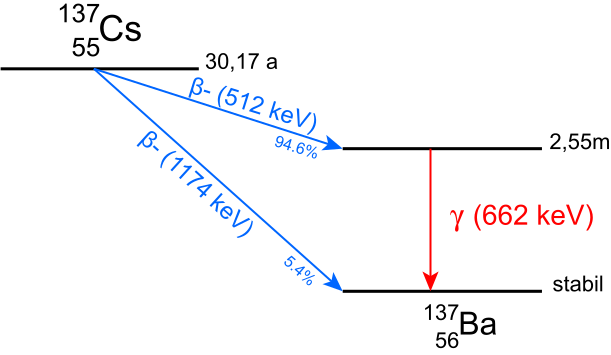
\includegraphics[width=0.75\textwidth]{zerfall.png}
  \caption{Zerfall eines $^{137} $Cs Atoms \cite{Zerfall}}
  \label{fig:zer}
\end{figure}


\subsection{Abschwächung}
Wenn Strahlung Materie durchdringt, wechselwirkt sie mit dieser. Dardurch verliert sie Energie und es wird von einer Abschwächung gesprochen.
Bei einer nicht kontinuierlichen Intensitätsverteilung kann die Intensitätsveränderung beschrieben werden durch 

\begin{equation}
  N = I_0 \text{exp} \left(- \sum_i \mu_i d_i \right) \, .
  \label{eqn:exp}
\end{equation}

Dabei sind $\mu_i$ die Absorptionskoeffizienten, $I_0$ die Eingansintensität und $d_i$ die Länge der Strecke, in welcher die Strahlung wechselwirkt. Dies 
lässt sich nun umstellen zu 

\begin{equation}
  \sum_i \mu_i d_i = \text{log} \left( \frac{I_0}{N_j}  \right) = I_i \, .
  \label{eqn:log}
\end{equation}

Hierbei steht $N_j$ für die jeweils gemessenen Ausgangsintensitäten, also der Intensität die nach dem Durchgang durch das Target gemessen wurde.
 Aus diesem Zusammenhang kann ein LGS (kurz für Lineares Gleichungssystem) aufgestellt werden.

\noindent
Da im Versuch ein 3x3-Würfel tomographisch untersucht wurde, kann eine 9 x 12 Matrix $\underline{\underline{A}}$ in dem Zusammenhang 

\begin{equation}
  \underline{\underline{A}} \vec{\mu} = \vec{I} 
  \label{eqn:matrix}
\end{equation}

aufgestellt werden. Das LGS wird bewusst überbestimmt aufgestellt (Mess-)Fehleranfälligkeiten zu senken, sodass die Matix (passend zu den Strahlengängen in der
\autoref{fig:projektion}) aussieht, wie in \autoref{fig:matrix} dargestellt ist.

\begin{figure}[H]
	\centering
	\begin{subfigure}[b]{0.45\textwidth}
		\centering
		\includegraphics[width=4.5cm]{matrix.png}
		\caption{Matrix A}
    \label{fig:matrix}
	\end{subfigure}
	~
	\begin{subfigure}[b]{0.45\textwidth}
		\centering
		\includegraphics[width=4.5cm]{projektion.png}
		\caption{Schematische Darstellung der Strahlengänge durch den Würfel}
    \label{fig:projektion}
	\end{subfigure}
\end{figure}

